\chapter{Klasyfikacja danych}

 Człowiek od zawsze próbuje skategoryzować i uporządkować posiadaną wiedzę w zbiory pozwalające na łatwy dostęp do przechowywanych informacji na przykład w sposób tabelaryczny.\ Klasyfikacja to proces rozpoznawania obiektów na bazie analizy ich cech.\ Jest to jedna z pierwszych rzeczy, której uczą się niemowlęta: rozróżniania kształtów, kolorów czy własnych rodziców. \ W póżniejszych latach te umiejętności są bardzo ważne, ponieważ w otaczającym świecie wiele rzeczy jest sklasyfikowanych.\ Przykładem takiej klasyfikacji są książki w katalogach bibliotecznych czy produkty spożywcze według jakości produkcji.
\\ \\
W uczeniu maszynowym klasyfikacja jest to metoda uczenia nadzorowanego, podczas której model próbuje przewidzieć etykietę obiektu na podstawie jego cech.\ Proces uczenia modelu klasyfikacji jest oparty o dwa zbiory, treningowy i testowy.\ Zbiór treningowy powinien być mniejszy od zbioru testowego.\ Po udanym procesie trenowania modelu następuje proces testowania, na podstawie którego wylicza się odpowiednie metryki pozwalające na ewaluacje modelu.\ W pracy magisterskiej wykorzystano zbiór danych, który posiada dwa typy etykiet [0, 1], dlatego też na tej podstawie zbudowano macierz pomyłek.

\section{Metryki klasyfikacji danych}
W trakcie ewaluacji algorytmu służącego do klasyfikacji wykorzystuje się metryki klasyfikacji.\ Służą one do przewidywanie etykiet klas na podstawie danych wejściowych.\ W zależności od ilości klas wyjściowych rozróżniamy klasyfikację binarną i wieloklasową.\ W klasyfikacji binarnej występują tylko dwie klasy wyjściowe, a w klasyfikacji wieloklasowej już tych klas jest więcej.\ Przykładem klasyfikacji binarnej jest np. wykrywanie niechcianych wiadomości w skrzynce mailowej.\ Wiadomość przychodzącą możemy określić jako 1 - \textit{,,pozytywną''}, bądź 0 - \textit{,,negatywną''}.\ Istnieje wiele sposobów na oceny klasyfikacji, do których zaliczamy między innymi dokładność, macierz pomyłek czy precyzję~\cite{Agrawal2024}.
\\ \\
Macierz pomyłek pokazuje jakie wyniki możemy otrzymać w procesie klasyfikacji.\ \refsource{Tabela}{tab:matrix-tn} obrazuje schemat macierzy pomyłek.\ Jest to miara wydajności problemów klasyfikacji.

\begin{table}[H]
    \centering
    \captionsource{Macierz pomyłek}{Opracowanie własne}
    \label{tab:matrix-tn}
    \begin{tabular}{|c|c|M{16mm}|M{16mm}|}
        \hline
         & & \multicolumn{2}{c|}{\textbf{Prawdziwe wartości}} \\ \hline
         & & \textbf{1} & \textbf{0} \\ \hline
        \rule{0pt}{13mm} \multirow{2}{*}{\rotatebox[origin=c]{90}{\parbox{18mm}{\textbf{Przewidziane wartości}}}} & \textbf{1} & \cellcolor{lightgreen}TP & \cellcolor{lightred}FN \\ \cline{2-4}
        \rule{0pt}{13mm} & \textbf{0} & \cellcolor{lightred}FP & \cellcolor{lightgreen}TN \\ \hline
    \end{tabular}
\end{table}
    Wyróżniamy 4 rodzaje rezultatów:
    \begin{itemize}
        \item  \textbf{TP} - prawdziwie pozytywny - przewidywano pozytywny wynik i otrzymano pozytywny wynik,
        \item \textbf{FN} - fałszywie negatywny - przewidywano negatywny wynik, a otrzymano pozytywny wynik,
        \item \textbf{FP} - fałszywie pozytywny - przewidywano pozytywny wynik, a otrzymano negatywny wynik,
        \item \textbf{TN} - prawdziwie negatywny - przewidywano negatywny wynik i otrzymano negatywny wynik.
    \end{itemize}

Opierając się o macierz pomyłek można wyznaczyć następujące metryki:
\begin{itemize}
    \item dokładność,
    \item precyzję,
    \item czułość,
    \item F1
    \item swoistość
    \item ROC - AUC~\cite{Agrawal2024}
\end{itemize}

\subsection{Dokładność}
\begin{equation}\label{math:acc}
    \frac{TP + TN}{TP + TN + FP + FN}
\end{equation}
Dokładność określa częstość poprawnego przewidywania klasyfikatora.\ Jest to stosunek wszystkich dobrze oznaczonych obiektów do liczby wszystkich prób~\cite{Agrawal2024, Blyszcz2022, Kulkarni2020}.

\subsection{Precyzja}
\begin{equation}\label{math:prec}
    \frac{TP}{TP + FP}
\end{equation}
Precyzja wyjaśnia ile z prawidłowo przewidzianych przypadków jest poprawnych.\ Jest to stosunek poprawnie wybranych obiektów klasy ,,\textit{1}'', do wszystkich wybranych obiektów tej klasy.\ Znajduje zastosowanie w przypadkach gdy wynik fałszywie dodatni jest większym problemem niż fałszywie ujemny~\cite{Agrawal2024, Blyszcz2022, Kulkarni2020}.

\subsection{Czułość}
\begin{equation}\label{math:rec}
    \frac{TP}{TP + FN}
\end{equation}
Czułość określia ile rzeczywistych pozytywnych przypadków byliśmy w stanie poprawnie przewidzieć za pomocą naszego modelu.\ Jest to stosunek poprawnie sklasyfikowanych obiektów klasy ,,\textit{1}'', do wszystkich obiektów, które powinny być w tej klasie.\ Czułość jest przydatną metryką w przypadkach gdy wynik fałszywie ujemny ma większe znaczenie niż wynik fałszywie dodatni~\cite{Agrawal2024, Blyszcz2022, Kulkarni2020}.

\subsection{Swoistość}
\begin{equation}\label{math:swo}
    \frac{TN}{TN + FP}
\end{equation}
Swoistość lub specyficzność pozwala określić ile rzeczywiście uzyskało się przypadków negatywnych.\ Jest to stosunek poprawnie zaklasyfikowanych obiektów klasy ,,\textit{0}'', do wszystkich obiektów, które powinny być w tej klasie~\cite{Agrawal2024}.

\subsection{F1}
\begin{equation}\label{math:f1}
   \frac{2*x*y}{x + y}
\end{equation}
Parametr F1 pozwala na połączoną ocenę precyzji i czułości.\ Jest to średnia harmoniczna precyzji (\textit{x}) i czułości (\textit{y}). Parametr F1 może być skuteczną metryką oceny w następujących przypadkach:
\begin{itemize}
    \item wyniki fałszywie pozytywne i fałszywie negatywne są równie kosztowne
    \item zwiększenie ilości danych nie zmienia skuteczności wyniku
    \item wynik prawdziwie ujemny jest wysoki~\cite{Agrawal2024}.
\end{itemize}

\subsection{ROC - AUC}
Krzywa ROC-AUC przedstawiona na \refsource{rysunku}{fig:roc-auc}, pozwala na ocenę sprawności klasyfikatora.\ ROC jest krzywą prawdopodobieństwa, którą wykreśla czułość w stosunku do swoistości.\ Wykres przedstawia wydajność (dokładność predykcji) modelu klasyfikacji.\ AUC \textit{(ang. Area Under Roc Curve)} jest to pole pod krzywą ROC.\ AUC to miara zdolności klasyfikatora do rozróżniania klas.

\begin{figure}[H]
    \centering
    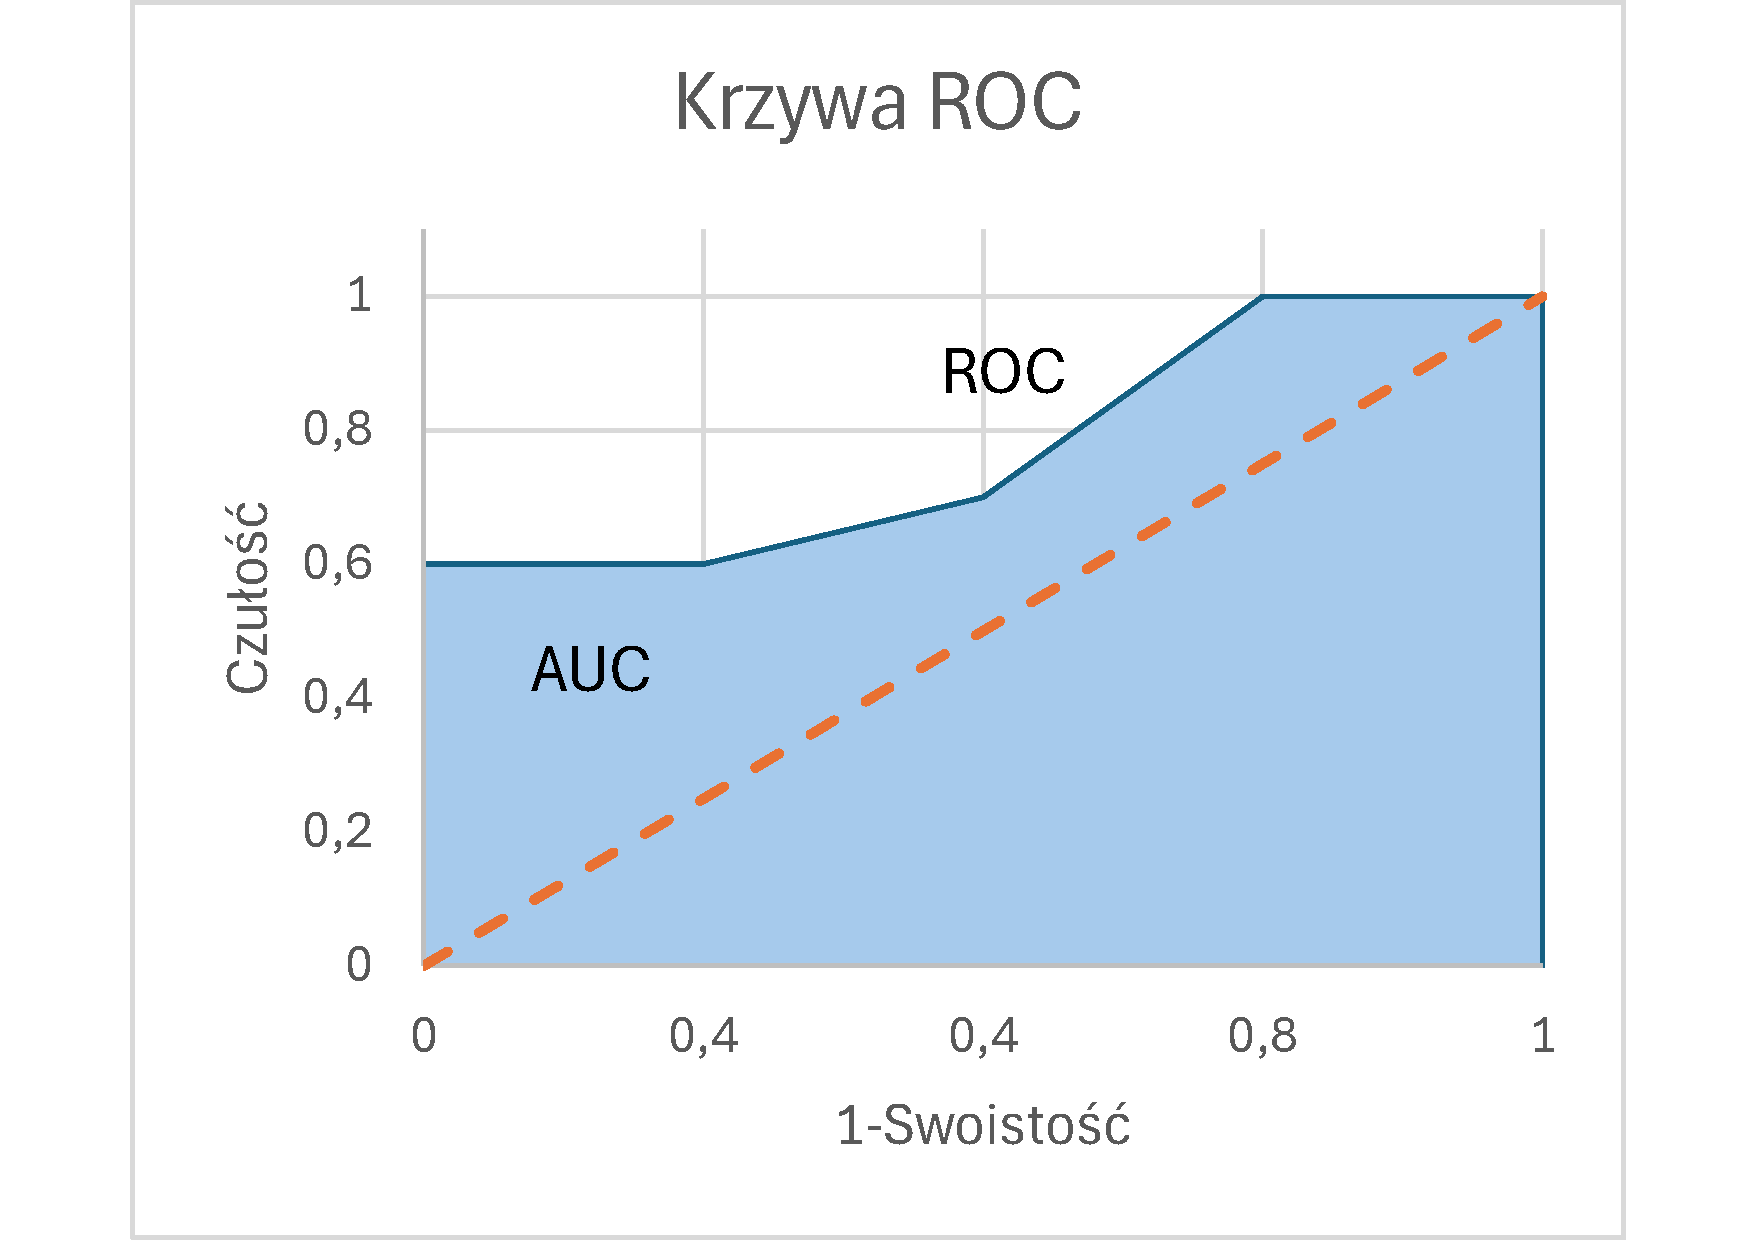
\includegraphics[width=0.8\textwidth]{images/roc-auc}
    \captionsource{Przykład krzywej ROC}{Opracowanie własne}
    \label{fig:roc-auc}
\end{figure}

Im większa jest wartość AUC tym lepsza wydajność modelu w rozróżnianiu klas pozytywnych i negatywnych.\ Wynik AUC jest z zakresu $[0, 1]$:
\begin{itemize}
    \item AUC = 1 - klasyfikator idealny, który rozróżnia wszystkie punkty,
    \item 0,5 < AUC < 1 - klasyfikator prawie idealny, czyli z dużym prawdopodobieństwem sklasyfikuje poprawnie obiekty
    \item AUC = 0,5 - klasyfikator losowy, oznacza to, że nie ma pewności czy klasyfikator jest w stanie rozpoznać cechy, czy może przypisuje je losowo,
    \item AUC < 0,5 - klasyfikator gorszy niż klasyfikator losowy~\cite{Algolytics, Agrawal2024}.
\end{itemize}